\section{Transport}
\begin{frame} {Resistive Plasma Diffusion}
  \begin{itemize}
    \item Resistive diffusion coefficient
          \[ D = \frac{\eta_\perp\beta}{2\mu_0} \sim \frac{\rho}{\tau} = D_c \]
          where $\rho$ and $\tau$ are step length and step time from classical random walk model.
    \item Resistive diffusion gives diffusion coefficient similar to classical result $D_c$.
  \end{itemize}
\end{frame}

\begin{frame} {Banana/Plateau/Pfirsch-Schl\"{u}ter Transport}
  \begin{itemize}
    \item Classical diffusion coefficient is $ D_{c} = \rho^{2}\nu $, where $\rho$ is the random walk length, and $\nu$ is the collision frequency.
    \item Plateau diffusion coefficient
          \[ D \sim \frac{v_{\parallel}}{v_{T}}v_{d}^{2} \frac{Rq}{v_{\parallel}} \sim \frac{v_{T}q}{R}\rho^{2} \]
  \end{itemize}

  \begin{figure}
    \centering
    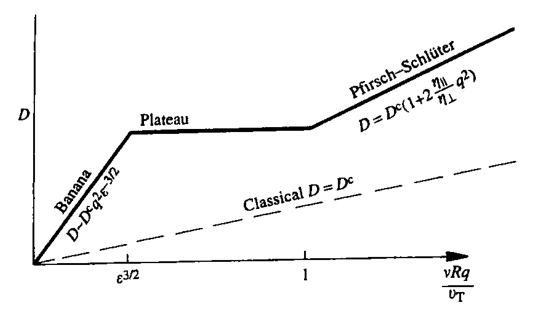
\includegraphics[width=0.6\textwidth]{figures/plateau-transport.png}
    \caption{Variation of diffusion coefficient with collision frequency.}
    \label{fig:plateau-transport}
  \end{figure}
\end{frame}

\begin{frame} {Ripple Transport}
  \begin{itemize}
    \item The finite number of toroidal field coils destroys the perfect axisymmetry of the device.
    \item Particles are trapped / lose energies to the "ripple well".
  \end{itemize}
  \begin{figure}
    \centering
    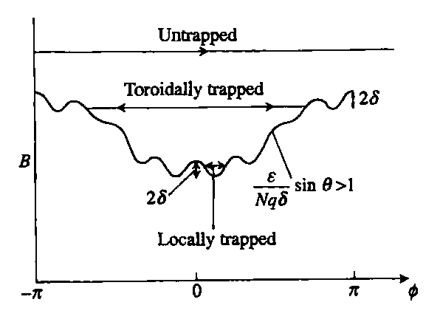
\includegraphics[width=0.5\textwidth]{figures/ripple-transport.png}
    \caption{Variation of magnetic field strength along a field line in a tokamak with a rippled field, and the resulting types of particle trapping.}
    \label{fig:ripple-transport}
  \end{figure}
\end{frame}
